\documentclass{article}
\usepackage{hyperref}
\usepackage{tabularx}
\usepackage{graphicx}
\usepackage{enumerate}
\usepackage{listings} 
\usepackage{float}

\begin{document}

\title{11-792 Project Report}
 
\author{Nicholas Gekakis, Boyue Li}
 
\maketitle
 
\section{Overview}

In this project, we are building a distributed question answering pipeline framework,
which allows users to easily configure multiple modules,
create complex pipelines and tune parameters automatically.

\section{Requirements}

    \subsection{Easy to configure and deploy}
    The framework should be easy to configure and deploy.

    \subsection{Save and resume}
    The framework should be save intermediate results so that it can be interrupted resume running at a later time.

    \subsection{Automatical parameter tuning}
    The framework should be able to automatically tune some parameters that have been exposed to the system by the pipeline developers.

    \subsection{Distributed parallel processing}
    The framework should support distributed parallel processing to handle large datasets and complicated pipelines (e.g. pipelines with several components).

    \subsection{Automatical load balancing}
    The framework should automatically handle load balancing since different modules need different excution time.

\section{Design}

    \subsection{Overview}

    As shown in Fig. \ref{fig:flow},
    a pipeline is constructed from several independent modules.
    A module reads data from data server,
    processes data according to all possible parameters,
    then save results for each configuration to the data server.

    The number of instances of each module is managed by the load balancing server.

    \begin{figure}[h]
        \begin{center}
            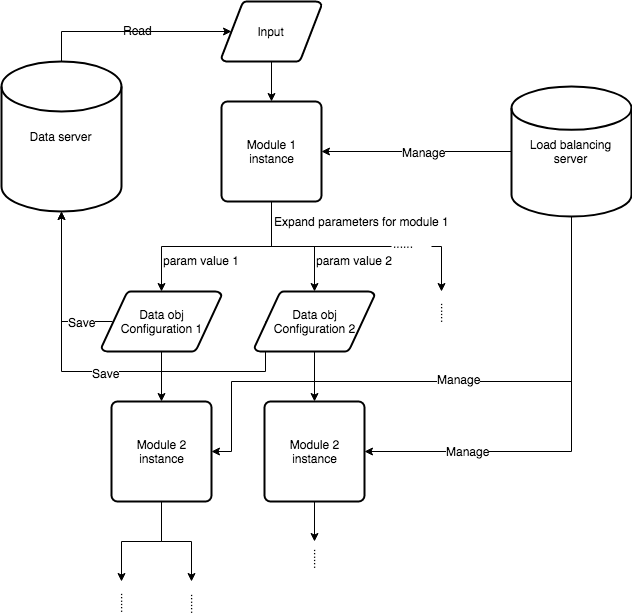
\includegraphics[width=\textwidth]{fig/flow.png}
        \end{center}
        \label{fig:flow}
        \caption{Execution flowchart.}
    \end{figure}

    Every module runs on an independent process,
    and communicates through RabbitMQ using data objects which contains parameters, current excuetion status and the path to input file.

    Users only need to specify
    \begin{enumerate}
        \item The connections between modules
        \item The parameters every module needs
    \end{enumerate}
    The framework will automatically handle execution, load balancing and parameter tuning.

    \begin{figure}[H]
        \begin{center}
            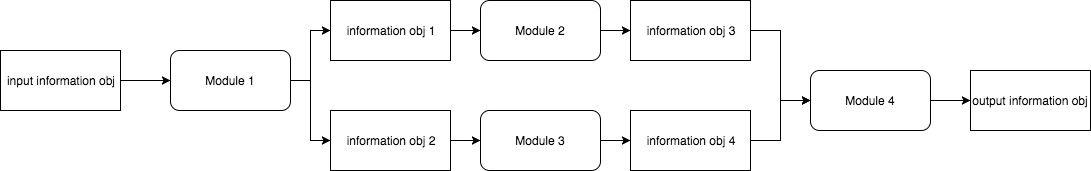
\includegraphics[width=1.2\textwidth]{fig/sample_pipeline.png}
        \end{center}
        \label{fig:sample_pipeline}
        \caption{A sample pipeline}
    \end{figure}
    Figure \ref{fig:sample_pipeline} shows a sample pipeline which passes the input information object
    through some modules and produces the output information object.



    \subsection{Pipeline}
    The pipeline class manages modules and parameters.
    It reads configuration file, creates the pipeline and controls load balancing when running.

    \begin{figure}[h]
        \begin{center}
            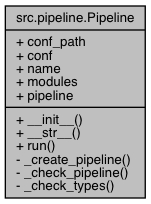
\includegraphics[width=0.3\textwidth]{fig/pipeline_uml.png}
        \end{center}
        \label{fig:pipeline_uml}
        \caption{UML diagram for the pipeline class.}
    \end{figure}

    \subsection{Module}
    A module is the basic computation unit which takes an input and produces an output.
    Every input and output is an information object defined in sec. \ref{sec:infomation_object}.

    A module needs to maintain the following fileds:
    \begin{itemize}
        \item Name of the module.
        \item Input module.
        \item Output module.
        \item Parameters.
        \item Configuration of the pipeline.
    \end{itemize}

    \begin{figure}[H]
        \begin{center}
            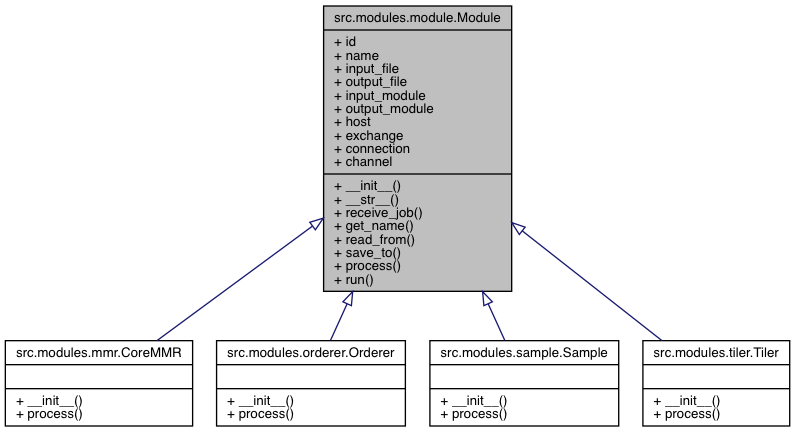
\includegraphics[width=\textwidth]{fig/module_uml.png}
        \end{center}
        \label{fig:module_uml}
        \caption{UML diagrams for the abstract module class and derived classes.}
    \end{figure}

    \subsection{Parameter}
    \label{sec:parameter}
    The parameter class manages one parameter.
    It should handle all operations related the parameter,
    including updating the parameter value according to its step size,
    set and reset the value.

    It also needs to save maintain the following fileds:
    \begin{itemize}
        \item Name of the parameter.
        \item Default values of the parameter.
        \item Tuning interval of the parameter.
        \item Step size of the parameter.
    \end{itemize}

    \begin{figure}[H]
        \begin{center}
            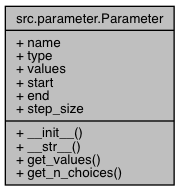
\includegraphics[width=0.3\textwidth]{fig/param_uml.png}
        \end{center}
        \label{fig:param_uml}
        \caption{UML diagram for parameter class.}
    \end{figure}

    \subsection{Data}
    \label{sec:infomation_object}
    The data class is the information object used to pass data between modules.
    It maintains the following fileds:
    \begin{itemize}
        \item Producing module: the module that produced this information object.
        \item Consuming module: the module that this information object to be passed to.
        \item Data path: the path to actual data file.
        \item Configuration: the configuration that produced the data object.
    \end{itemize}

    \subsection{File format}
    A data file has a description contains the following fileds:
    \begin{itemize}
        \item Data: the actual data.
        \item Configuration: the configuration produced the file it.
        \item Timestamp: the timestamp when it is created.
        \item Producing module: the module that produced this file.
    \end{itemize}


    \subsection{Dataset}
    Datasets are handled by the dataset class.

    \begin{figure}[H]
        \begin{center}
            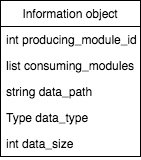
\includegraphics[width=0.3\textwidth]{fig/dataset_uml.png}
        \end{center}
        \label{fig:dataset_uml}
        \caption{UML diagram for the dataset class.}
    \end{figure}

    \subsection{Configuration file}
    We use YAML files to configure the framework.


\section{Example pipeline}

\section{Experiments}
    \subsection{Dataset1}
    \subsection{Dataset2}
    \subsection{Dataset3}

\section{Conclusion}

\section*{Acknowledgements}

\end{document}



